\documentclass[11pt, english]{article}
%\usepackage[latin1]{inputenc}
\usepackage[T1]{fontenc}
\usepackage[utf8x]{inputenc}
\usepackage[english]{babel}   % S P R A A K
% \usepackage{graphicx}    % postscript graphics
\usepackage{amssymb, amsmath, amsthm, amssymb} % symboler, osv
\usepackage{mathrsfs}
\usepackage{url}
\usepackage{thmtools}
\usepackage{enumerate}  % lister $  
\usepackage{float}
\usepackage{tikz}
\usepackage{tikz-cd}
\usetikzlibrary{calc}
%\usepackage{tikz-3dplot}
\usepackage{subcaption}
\usepackage[all]{xy}   % for comm.diagram
\usepackage{wrapfig} % for float right
\usepackage{hyperref}
\usepackage{mystyle} % stilfilen      

%\usepackage[a5paper,margin=0.5in]{geometry}


\begin{document}
\title{Two constructions}
\date{}
\maketitle

We give two smoothings of a singular Calabi-manifold $X_0$, both with actions of $D_6$, the symmetries of the hexagon.

\begin{lemma}
There is an isomorphism $S_3 \times \Z_2 \simeq D_6$.
\end{lemma}
\begin{proof}
Let $D_6 = \langle \rho, \sigma \mid \rho^6=\sigma^2=s\rho s \rho \rangle$. Then $S_3 \simeq \langle \rho^2, \sigma \rangle $ and $\mathbb Z^2 \simeq \langle \rho ^3 \rangle$.
\end{proof}

\subsection{Construction 1}

Let $E$ be a 3-dimensional vector space. Let $\{e_1,e_2,e_3\}$ be a basis for $E$. Then $S_3$ act on $E$ by $e_i \mapsto e_{\sigma(i)}$. It also act on $(E \otimes E)^{\oplus 2)}\approx k^{18}$. There is a $\Z_2$-action switching the factors. Let $\PP=\PP(k^{18})$. Then $S_3 \times \Z_2$ act on $\PP$. 

The elements of $\PP$ are pairs of $3 \times 3$-matrices, not both zero. Let $M$ be the closure of the set of pairs $(A,B)$ where $\rank A = \rank B = 1$. 

If $\PP$ have coordinates $x_1,\ldots,x_{18}$, let $M_1, M_2$ be generic matrices:
\[
M_1 = \begin{pmatrix}
x_1 & x_2 & x_3 \\
x_4 & x_5 & x_6 \\
x_7 & x_8 & x_9 
\end{pmatrix}\,
\text{ and }
M_1 = \begin{pmatrix}
x_{10} & x_{11} & x_{12} \\
x_{13} & x_{14} & x_{15} \\
x_{16} & x_{16} & x_{17}
\end{pmatrix}.
\]

Then $M$ is defined by the zeroes of the $2 \times 2$-minors of $M_1$ and $M_2$. Note that $M$ is the projective join of $\mathbb P^2 \times \mathbb P^2 \hookrightarrow \mathbb P^8$. 

The variety $M$ is $9$-dimensional: the affine cone over $M$, $C(M)$, is equal to $C(\mathbb P^2 \times \PP^2) \times C(\mathbb P^2 \times \PP^2)$. This variety has dimension $5+5=10$, hence its projectivization $M$ is $9$-dimensional. 

The singular locus of $M$ consists of the pairs $(0,B)$, and $(A,0)$, where $\rank A= \rank B = 1$, hence $\dim \Sing M = 4$.

Intersecting $M$ with a codimension $6$ hyperplane gives a smooth Calabi-Yau variety $X_1$. It has topological Euler characteristic $-72$. 


%%%% SECOND CONSTRUCTION
%%%%
\subsection{Construction 2}

Let $E$ be a $2$-dimensional vector space with basis $\{e_1,e_2\}$. Let $\PP=\PP\left((E \otimes E \otimes E)^{\oplus 2}\right)$. Then $\PP=\PP^{15}$. There is an action of $S_3$ on $E \otimes E \otimes E$ given by permuting the tensor factors. Combining this with a $\Z_2$ switching $A$ and $B$, we get a $S_3 \times \Z \simeq D_6$-action on $\PP$. 

The elements of $\PP$ are pairs $(A,B)$ of $2 \times 2 \times 2$-tensors, not both zero. 

Let $N$ be the closure of set of pairs $(A,B)$ where both $A$ and $B$ have tensor rank $1$\footnote{An elements of $E^\otimes 3$ have rank $1$ if it is a pure tensor. It has rank $k$ if it can be written as a sum of $k$ pure tensors.}. A pure $2 \times 2 \times 2$-tensor can be visualized as a box in $\Z^3$ of unit volume. Let the variables on $\PP$ be $a_{ijk}$ and $b_{ijk}$ for $i,j,k=0,1$. See the diagram in \figref{222tensor}.

\begin{figure}
\centering
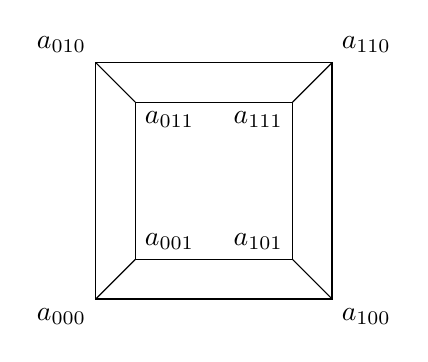
\begin{tikzpicture}
\draw (0,0) -- (3,0) -- (3,3) -- (0,3) -- cycle;
\draw (0.5,0.5) -- (2.5,0.5) -- (2.5,2.5) -- (0.5,2.5) -- cycle;
\draw (0,0) -- (0.5,0.5);
\draw (3,0) -- (2.5,0.5);
\draw (3,3) -- (2.5,2.5);
\draw (0,3) -- (0.5,2.5);
\node[below left] at (0,0) {$a_{000}$};
\node[below right] at (3,0) {$a_{100}$};
\node[above right] at (3,3) {$a_{110}$};
\node[above left] at (0,3) {$a_{010}$};

\node[above right] at (0.5,0.5) {$a_{001}$};
\node[above left] at (2.5,0.5) {$a_{101}$};
\node[below left] at (2.5,2.5) {$a_{111}$};
\node[below right] at (0.5,2.5) {$a_{011}$};
\end{tikzpicture}
\caption{A $2 \times 2 \times 2$-tensor.}
\label{fig:222tensor}
\end{figure}

The equations of the set of rank $1$ tensors are obtained as the ''minors'' along the $6$ sides together with the minors along the $4$ long diagonals, giving a total of $9$ binomial equations. 

Note that $N$ is the projective join of two copies of $\PP^1 \times \PP^1 \times \PP^1$.

The singular locus of $N$ consists of the pairs $(A,0)$ and $(0,B)$ where both $A,B$ have rank $1$. Hence the singular locus is of dimension $3$.

Intersecting $N$ with a codimension $4$-hyperplane gives a smooth variety $X_2$. It is Calabi-Yau and has topological Euler characteristic $-48$.

\subsection{A Calabi-Yau with isolated singularities}

Let $\dP6 \subset \PP^6$ be the del Pezzo surface of degree $6$ anticanonically embedded in $\PP^6$.

Let us describe two embeddings of $\dP6$ into $\PP^2 \times \PP^2$ and $(\PP^1)^{\times 3}$, respectively. The surface $\dP6$ is the blowup of $\PP^2$ in three points. Assume these are $P_1=(1:0:0)$, $P_2= (0:1:0)$ and $P_3=(0:0:1)$.

Then we can realize $\dP6$ as the solutions of the matrix equation
\[
\begin{pmatrix}
0 & a_0 & -a_1 \\  % r a_0 s a_1
b_1 & 0 & -b_0 \\
c_0 & -c_1 & 0
\end{pmatrix}
\begin{pmatrix}
x_0 \\ x_1 \\ x_2
\end{pmatrix} = 0
\]
in $\mathbb P^2 \times \PP^1 \times \PP^1 \times \PP^1$. Since the $r_i,s_i$ are variables in $\PP^1$, we see that the matrix cannot have rank $1$. Hence the matrix have rank exactly $2$, and that the matrix equation is equivalent to the equation $\det M =a_0b_0c_0-a_1b_1c_1= 0$ in $(\PP^1)^3$. Hence $\dP6$ is the set of zeroes of a section of $\OO_{(\PP^1)^3}(1,1,1)$.

We can also describe $\dP6$ as the closure of the graph of a rational map. The ideal of the three points is $(x_1x_2,x_0x_2,x_1x_2)$, and this gives a rational map $f: \PP^2 \rmap  \PP^2$ by $(x_0:x_1:x_2) \mapsto (x_1x_2:x_0x_2:x_0x_1)$. The blowup is defined as the closure of the graph of this map, and lives inside $\PP^2_{x_0x_1x_2} \times \PP^2_{y_0y_1y_2}$ as the solutions of the equation $x_0y_0=x_1y_1=x_2y_2$. Hence $\dP6$ is the zero locus of a section of $\mathscr O_{\PP^2 \times \PP^2}(1,1)^{\oplus 2}$.

In these descriptions, we can think of $\dP6$ as either the set of pure $2 \times 2 \times 2$ tensors with two opposite corners (recall \figref{222tensor}) equal, or as the set of rank $1$ matrices with all the diagonal entries equal.

Now consider $M_1$ from above. It is the join of two copies of $\PP^2 \times \PP^2$. Now let $h_1=x_1-x_5,h_2=x_1-x_9,h_3=x_{10}-x_{14}$ and $h_4=x_{10}-x_{17}$. By the description above, we see that variety $M_1 \cap V(h_1,h_2,h_3,h_4)$ is the join of two copies of $\dP6$. The singular locus is the disjoint union of these two. Intersecting with two more generic hyperplanes we get a Calabi-Yau $X_0$ with $12$ isolated singularities. A local calculation shows that these singularities are locally isomorphic to $C(\dP6)$, the affine cone over a del Pezzo. 

Consider now $M_2$ from above. It is the join of two copies of $(\PP^1)^3$. Let $g_1=a_{000}-a_{111}$ and $g_2=b_{000}-b_{111}$. Then $M_2 \cap V(g_1,g_2)$ is again the join of two copies of $\dP6$, isomorphic to the one above by a coordinate renaming.

Perturbing the $h_i$ or the $g_i$ by generic linear equations we get $X_1$ and $X_2$.

Hence we see that $X_1,X_2$ both degenerate to the same singular Calabi-Yau variety.

\subsection{Euler characteristic heuristics}

Let $\hat X$ be the blowup of $X_0$ in the 12 singular points. The exceptional divisors are del Pezzo surfaces. 

One can show that $C(\dP6)$ has two topological different smoothings $V_1,V_2$, where $V_1 = \PP^2 \times \PP^2 \bs \dP6$ and $V_2=(\PP^1)^3 \bs \dP6$. The Euler characteristics are $0$ and $2$, respectively.

Let us for the moment assume without proof that $X_1$ is what is obtained when we replace all the singularities in $X_0$ by $V_1$, and similarly for $X_2$.

Let $U = X_0 \bs \Sing(X_0)$. Then in the first case, we have $\chi(X_1)=\chi(U)+12\chi(V_1)=\chi(U)+12\cdot 0 = \chi(U)=-72$. 

One the other hand, we have $\chi(X_2)=\chi(U)+12\chi(V_2)=\chi(U)+12\cdot 2 =-48$, implying $\chi(U)=-72$, so the calculations are at least consistent.

In both cases, we find that $\chi(\hat X)=0$.

It would be interesting to see if we can find a crepant resolution. Also, can we use this resolution to find the Hodge numbers of $X_1$ and $X_2$?

\end{document}